\documentclass{article}
\usepackage[utf8]{inputenc}
\title{Lecture 9 Decision  Trees}
\author{wbg231 }
\date{December 2022}
\newcommand{\R}{$\mathbb{R}$}
\newcommand{\B}{$\beta$}
\newcommand{\A}{$\alpha$}
\newcommand{\D}{\Delta}

\newcommand{\avector}[2]{(#1_2,\ldots,#1_{#2})}
\newcommand{\makedef}[2]{$\textbf{#1}$:#2 }
\usepackage{tikz,graphicx,hyperref,amsmath,amsfonts,amscd,amssymb,bm,cite,epsfig,epsf,url}

\begin{document}

\maketitle

\section*{introduction}
\begin{itemize}
\item Decision trees are an inherently non linear type of model
\item they are lso a good way to understand Ensemble  methods. 
\section*{Decision trees}
\item regression trees try to predict a continuous outcome 
\item classification trees try to predict a discrete class.
\item a binary tree has 2 children nodes there are also multi-way trees that have more 
\item each node contains a subset of teh data 
\item the data splits created by each node involve only a single feature 
\item for continuous variables the splits are always of the form $x_{i}\leq y$
\item for discrete variables we partition the values into two stets 
\item predictors are made in the leaf nodes 
\subsection*{constructing the tree }
\item our goal is to find the boxes $R_1\dots R_J$ that minimize
 $\Sigma_{j=1}^{J}\Sigma_{i\in R_{j}}(y_i-\hat{y}_{R_{j}})$ subject to 
 complexity constraints 
\item the issue with this is finding the true optimal binary tree is computationally
intractable
\item so instead we use a greedy algorithm  (that is we take the best choice at every step)
where we start at the root and on our first step take the splits that would 
result in the minimal loss, and then pass the data split like that to the next
step and have each for each of those sections pick the best splits
and continue this until we hit some stopping criteria
\item we only split regions defined in the last step at each current step 
we predict based on the mean value of a terminal node ie $\hat{y}_{R_{m}}=mean(y_i|x_i\in R_{m})$ 
\item so building a tree like this we are making the best local choice at every step but are unlikely to reach the overall optimal choice
\item \includegraphics*[width=10cm]{lecture_notes/lecture_9/immages/l9_1.png}
\item so the left is how the tree looks for regression 
\item each node, is a binary decision with a condition that splits the tree remaining data into 2 groups in the binary case 
\item the the right side, is the search space. as you can see node (that is condition) make s a linear subdivision of our search space. 
\item 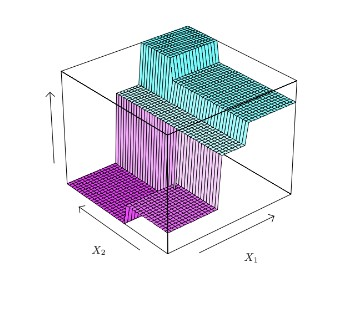
\includegraphics[width=10cm]{lecture_notes/lecture_9/immages/l9_2.jpg}
\item geometrically this looks like this kind of step wise division as can be seen in this chart. 
\subsection*{ finding the best split point}
\item there are infinitely many split points for each feature. 
\item suppose we have a vector $D=\{(x^1,y^1)...(x^n,y^n)\}$ where $x^i\in \mathbb{R}^{d}, y^i\in \mathbb{R}\forall i \in [1,n]$
\item suppose we are not considering splitting on the jth feature. ie $x^{i}_j$ 
\item we can sort our values by there value of the jth feature as $x_{j}(1)\cdots x_j(n)$
\item lets only consider split points between two adjacent values. note that any split point between the two same values will have the same loss.
\item due to this it is common to split half way between the two adjacent values $$s_j\in \{\frac{1}{2}(x_j(r)+x_{j}(r+1)|r=1\cdots n-1\}$$
so this is just saying that geometrically we are taking our split to be halfway between two adjacent points 
\subsection*{decision trees and over fitting}
\item 
\end{itemize}
\end{document}
